% Created 2023-04-01 Sat 19:51
% Intended LaTeX compiler: lualatex
\documentclass[bigger]{beamer}
\usepackage{graphicx}
\usepackage{longtable}
\usepackage{wrapfig}
\usepackage{rotating}
\usepackage[normalem]{ulem}
\usepackage{amsmath}
\usepackage{amssymb}
\usepackage{capt-of}
\usepackage{hyperref}
\usetheme[progressbar=foot, sectionpage=none, numbering=fraction]{metropolis}
\usepackage{tikz}
\usepackage{booktabs}
\usepackage{adjustbox}
\usepackage{diagbox}
\usepackage{latexcolors}
\usetikzlibrary{automata, positioning, arrows, arrows.meta}
\usepackage{diagbox}
\usepackage{dsfont}
\usepackage{fontawesome5}
\usepackage{color}
\usepackage{transparent}
\usepackage{textpos}
\usepackage{mathtools}
\usepackage[mathrm=sym]{unicode-math}
\definecolor{RedBrown}{RGB}{192, 4, 4} \setbeamercolor{progress bar}{fg=RedBrown} \setbeamercolor{title separator}{fg=RedBrown}
\setbeamercolor{progress bar in head/foot}{fg=RedBrown} \setbeamercolor{progress bar in section page}{fg=RedBrown} \setbeamercolor{alerted text}{fg=RedBrown}
\pretocmd{\tableofcontents}{\thispagestyle{empty}}{}{}
\addtocounter{framenumber}{-1}
\usepackage{listings}
\usepackage{xcolor}
\definecolor{codegreen}{rgb}{0,0.6,0}
\definecolor{codegray}{rgb}{0.5,0.5,0.5}
\definecolor{codepurple}{rgb}{0.58,0,0.82}
\definecolor{backcolour}{HTML}{f0f0f0}
\lstdefinestyle{mystyle}{
backgroundcolor=\color{backcolour},
commentstyle=\color{codegreen},
keywordstyle=\color{magenta},
numberstyle=\tiny\color{codegray},
stringstyle=\color{codepurple},
basicstyle=\ttfamily,
breakatwhitespace=false,
breaklines=true,
captionpos=b,
keepspaces=true,
numbers=none,
numbersep=5pt,
showspaces=false,
showstringspaces=false,
showtabs=false,
tabsize=2
}
\lstset{style=mystyle}
\usetheme{default}
\author{Andrea Pierré}
\date{April 4, 2023}
\title{Learning useful representations to solve a place-odor association task}
\institute{Fleischmann Lab}
\titlegraphic{\hfill\includegraphics[height=1.5cm]{img/Brown Logo_2016_2 Color Process ST_1300.png}\vspace{7em}\flushright\includegraphics[height=1.5cm]{img/qr-code.png}}
\setbeamercovered{transparent=10}
\hypersetup{
 pdfauthor={Andrea Pierré},
 pdftitle={Learning useful representations to solve a place-odor association task},
 pdfkeywords={},
 pdfsubject={},
 pdfcreator={Emacs 28.2 (Org mode 9.6)}, 
 pdflang={English}}
\begin{document}

\maketitle
\section{Context of the project}
\label{sec:org340210c}
\section*{Context}
\label{sec:orgecc459c}
{%
\setbeamertemplate{background canvas}{\includegraphics[height=\paperheight]{img/kitchen1.png}}
\begin{frame}[fragile]{Odor-place association}
\end{frame}
}
\section*{Context}
\label{sec:org7446d4d}
{%
\setbeamertemplate{background canvas}{\includegraphics[height=\paperheight]{img/kitchen2.png}}
\begin{frame}[fragile]{Odor-place association}
\addtocounter{framenumber}{-1}
\end{frame}
}
\section*{Context}
\label{sec:org3f2fab2}
{%
\setbeamertemplate{background canvas}{\includegraphics[height=\paperheight]{img/kitchen3.png}}
\begin{frame}[fragile]{Odor-place association}
\addtocounter{framenumber}{-1}
\end{frame}
}
\begin{frame}[label={sec:org81e9e0b}]{The LEC is key to sensory associations and spatial memory}
\begin{columns}
\begin{column}{0.45\columnwidth}
%\pause
%\scriptsize
%\footnotesize
\footnotesize
\begin{itemize}
\item \alert{Piriform} encodes olfactory information
\item \alert{Hippocampus} encodes spatial information
\item \alert{LEC} encodes both olfactory \& spatial information
\end{itemize}
\end{column}
\begin{column}{0.55\columnwidth}
\begin{center}
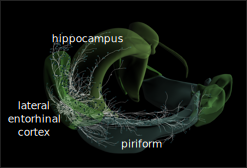
\includegraphics[width=\textwidth]{img/brain.png}
\end{center}
\end{column}
\end{columns}
\end{frame}

\begin{frame}[label={sec:org14896ea}]{Diamond arena experimental setup}
\begin{textblock}{5}(11,-1.3)
\center
\includegraphics[width=3em]{img/olivia.jpg}\\
\scriptsize
Olivia McKissick
\end{textblock}
\begin{center}
\includegraphics[width=0.8\textwidth]{img/physical-diamond-arena.png}
\end{center}
\end{frame}
\begin{frame}[label={sec:orge4039ce}]{Diamond arena olfactory task}
\begin{textblock}{5}(11,-0.5)
\center
\includegraphics[width=3em]{img/olivia.jpg}\\
\scriptsize
Olivia McKissick
\end{textblock}
\begin{columns}
\begin{column}[t]{0.5\columnwidth}
\center
Allocentric\\
(go west/east)
\begin{center}
\includegraphics[width=0.8\textwidth]{img/allocentric-task.png}
\end{center}
\end{column}

\begin{column}[t]{0.5\columnwidth}
\center
Egocentric\\
(go right/left)
\begin{center}
\includegraphics[width=0.8\textwidth]{img/egocentric-task.png}
\end{center}
\end{column}
\end{columns}
\end{frame}

\begin{frame}[<+->][label={sec:orga88f906}]{What is Reinforcement Learning and why use it ?}
\begin{columns}
\begin{column}{0.55\columnwidth}
% \usepackage{fontawesome5}
\usetikzlibrary{positioning,fit,arrows}


\tikzset{
    %Define standard arrow tip
    >=latex,
    %Define style for boxes
    punkt/.style={
           rectangle,
           rounded corners,
           draw=black, very thick,
           text width=7.5em,
           minimum height=2em,
           text centered},
    % Define arrow style
    pil/.style={
           ->,
           thick,}
}

\begin{adjustbox}{max width=\columnwidth, keepaspectratio}
    \begin{tikzpicture}[node distance=3em, auto,]
     %nodes
        \node (center) {};
        \node[punkt, above=of center] (agent) {Agent \faIcon{robot}};
        \node[punkt,below=of center] (environment) {Environment \faIcon{globe}};
        \node[right=8em of center, align=center] (action) {Action\\$a_t$};
        \node[left=8em of center, align=center] (state_reward) {State, Reward\\$s_t$, $r_t$};

        \path[pil]
        (state_reward.east) edge [->, bend left=45] node {} (agent.west)
        (environment.west) edge [- , bend left=45] node {} (state_reward.east)
        (action.west) edge [->, bend left=45] node {} (environment.east)
        (agent.east) edge [-, bend left=45] node {} (action.west);
    \end{tikzpicture}
\end{adjustbox}
\end{column}

\begin{column}{0.45\columnwidth}
\footnotesize
\begin{itemize}
\item Theoretical framework hypothesized to be implemented in the brain
\item Tool to model behavior
\item Goal of the agent : maximize rewards
\item Natural fit for behavioral experiments involving rewards and learning
\end{itemize}
\end{column}
\end{columns}
\end{frame}

\begin{frame}[label={sec:orgd153469}]{RL maps states to optimized actions}
\begin{columns}
\begin{column}{0.5\columnwidth}
\begin{center}
\includegraphics[height=0.8\textheight]{./img/RL_mapping.drawio.png}
\end{center}
\end{column}
\begin{column}{0.5\columnwidth}
\begin{adjustbox}{max width=\columnwidth, keepaspectratio}
\( Q^{new}(s_t, a_t) \longleftarrow Q(s_t, a_t) + \underbrace{\alpha}_\text{learning rate}\overbrace{(\underbrace{r_t}_\text{reward} + \gamma \operatorname*{max}_a Q(s_{t+1, a}) - Q(s_t, a_t))}^\text{temporal difference} \)
\end{adjustbox}\\[1em]
\begin{adjustbox}{max width=\columnwidth, keepaspectratio}
%\begin{align}
\( \mathbf{Q} = \mathrm{\mathbf{x}} \cdot \mathbf{W} \)
%\end{align}
\end{adjustbox}
\end{column}
\end{columns}
\end{frame}
\section*{Question}
\label{sec:orgb21113c}
\begin{frame}[fragile]{}
\metroset{block=fill}
\begin{exampleblock}{Question}
Which representations are needed by the brain to learn a place-odor association task ?
\end{exampleblock}
\end{frame}
\section{Modeling \& preliminary results}
\label{sec:orgf8b37a7}
\begin{frame}[label={sec:orgcb19ad2}]{Allocentric vs. Egocentric}
\begin{columns}
\begin{column}{0.5\columnwidth}
\center
Allocentric
\end{column}
\begin{column}{0.5\columnwidth}
\center
Egocentric
\end{column}
\end{columns}
\begin{block}{~}
\begin{center}
\includegraphics[width=.9\linewidth]{img/ego-vs-allo.jpg}
\end{center}
\end{block}
\end{frame}
\begin{frame}[label={sec:org66ae1d2}]{The model}
\begin{columns}
\begin{column}{0.5\columnwidth}
\center
Allocentric
\begin{center}
\includegraphics[width=\textwidth]{img/RL_env-allo-model.drawio.png}
\end{center}
\end{column}
\begin{column}{0.5\columnwidth}
\end{column}
\end{columns}
\end{frame}
\begin{frame}[label={sec:org526b0a4}]{The model}
\addtocounter{framenumber}{-1}
\begin{columns}
\begin{column}{0.5\columnwidth}
\center
Allocentric
\begin{center}
\includegraphics[width=\textwidth]{img/RL_env-allo-model.drawio.png}
\end{center}
\end{column}
\begin{column}{0.5\columnwidth}
\center
Egocentric
\begin{center}
\includegraphics[width=\textwidth]{img/RL_env-ego-model.drawio.png}
\end{center}
\end{column}
\end{columns}
\end{frame}
\begin{frame}[label={sec:org304bd3f}]{The joint representation encodes odor + location}
\begin{center}
\includegraphics[width=.9\linewidth]{img/joint-repr.drawio.png}
\end{center}
\end{frame}
\begin{frame}[label={sec:orge5fcb56}]{Minimizing the number of steps to solve the task}
\begin{columns}
\begin{column}[t]{0.5\columnwidth}
\begin{center}
With joint representation
\end{center}
\begin{center}
\includegraphics[width=\textwidth]{img/steps-allo-joint-repr.png}
\end{center}
\(\to\) The agent learns to solve the task
\end{column}

\begin{column}[t]{0.5\columnwidth}
\begin{center}
Without joint representation
\end{center}
\begin{center}
\includegraphics[width=\textwidth]{img/steps-allo-no-joint-repr.png}
\end{center}
\(\to\) The agent doesn't learn
\end{column}
\end{columns}
\end{frame}
\begin{frame}[label={sec:org8c4df44}]{Maximizing rewards}
\begin{columns}
\begin{column}[t]{0.5\columnwidth}
\begin{center}
With joint representation
\end{center}
\begin{center}
\includegraphics[width=\textwidth]{img/rewards-allo-joint-repr.png}
\end{center}
\(\to\) The agent learns to solve the task
\end{column}

\begin{column}[t]{0.5\columnwidth}
\begin{center}
Without joint representation
\end{center}
\begin{center}
\includegraphics[width=\textwidth]{img/rewards-allo-no-joint-repr.png}
\end{center}
\(\to\) The agent doesn't learn
\end{column}
\end{columns}
\end{frame}
\begin{frame}[label={sec:org2230165}]{What policy did the agent learned ?}
\vspace{-7em}
\begin{columns}
\begin{column}[t]{0.5\columnwidth}
\begin{center}
\includegraphics[height=0.4\textheight]{img/policy-allo-north-light.png}
\end{center}
\end{column}
\begin{column}[t]{0.5\columnwidth}
\begin{center}
\includegraphics[height=0.4\textheight]{img/policy-allo-south-light.png}
\end{center}
\end{column}
\end{columns}
\end{frame}
\begin{frame}[label={sec:orgfd1915a}]{What policy did the agent learned ?}
\begin{columns}
\begin{column}[t]{0.5\columnwidth}
\begin{center}
\includegraphics[height=0.4\textheight]{img/policy-allo-north-light.png}
\end{center}
\begin{center}
\includegraphics[height=0.4\textheight]{img/policy-allo-odor-A.png}
\end{center}
\end{column}
\begin{column}[t]{0.5\columnwidth}
\begin{center}
\includegraphics[height=0.4\textheight]{img/policy-allo-south-light.png}
\end{center}
\begin{center}
\includegraphics[height=0.4\textheight]{img/policy-allo-odor-B.png}
\end{center}
\end{column}
\end{columns}
\end{frame}
\section{Next steps}
\label{sec:org51e70b8}
\begin{frame}[label={sec:orga46bf71}]{What we have done so far}
\center
% \usepackage{fontawesome5}
\usetikzlibrary{positioning,fit,arrows}


\tikzset{
    %Define standard arrow tip
    >=latex,
    %Define style for boxes
    punkt/.style={
           rectangle,
           rounded corners,
           draw=black, very thick,
           text width=7.5em,
           minimum height=2em,
           text centered},
    % Define arrow style
    pil/.style={
           ->,
           thick,}
}

\begin{adjustbox}{max height=0.95\textheight, keepaspectratio}
    \begin{tikzpicture}[node distance=3em, auto,]
     %nodes
        \node (center) {};
        \node[punkt, above=of center] (agent) {Agent \faIcon{robot}};
        % \node at (0,3.7) {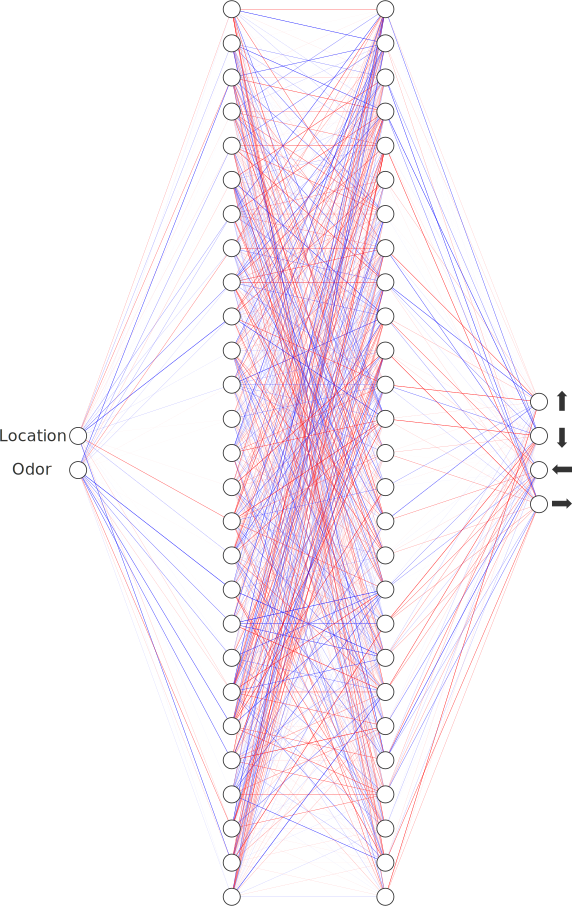
\includegraphics[height=6em]{./img/nn.svg.png}};
        \node [above=-0.2em of agent] {\includegraphics[height=8em]{./img/Q-table.png}};
        \node[punkt,below=of center] (environment) {Environment \faIcon{globe}};
        \node[right=8em of center, align=center] (action) {Action\\$a_t$};
        \node[left=8em of center, align=center] (state_reward) {State, Reward\\$s_t$, $r_t$};
        \node [below=-0.2em of environment] {\includegraphics[height=8em]{./img/RL_env-allo-model.drawio.png}};

        \path[pil]
        (state_reward.east) edge [->, bend left=45] node {} (agent.west)
        (environment.west) edge [- , bend left=45] node {} (state_reward.east)
        (action.west) edge [->, bend left=45] node {} (environment.east)
        (agent.east) edge [-, bend left=45] node {} (action.west);
    \end{tikzpicture}
\end{adjustbox}
\end{frame}

\begin{frame}[label={sec:orgecc53ea}]{From tabular RL to deep RL}
\center
\addtocounter{framenumber}{-1}
% \usepackage{fontawesome5}
\usetikzlibrary{positioning,fit,arrows}


\tikzset{
    %Define standard arrow tip
    >=latex,
    %Define style for boxes
    punkt/.style={
           rectangle,
           rounded corners,
           draw=black, very thick,
           text width=7.5em,
           minimum height=2em,
           text centered},
    % Define arrow style
    pil/.style={
           ->,
           thick,}
}

\begin{adjustbox}{max height=0.95\textheight, keepaspectratio}
    \begin{tikzpicture}[node distance=3em, auto,]
     %nodes
        \node (center) {};
        \node[punkt, above=of center] (agent) {Agent \faIcon{robot}};
        % \node at (0,3.7) {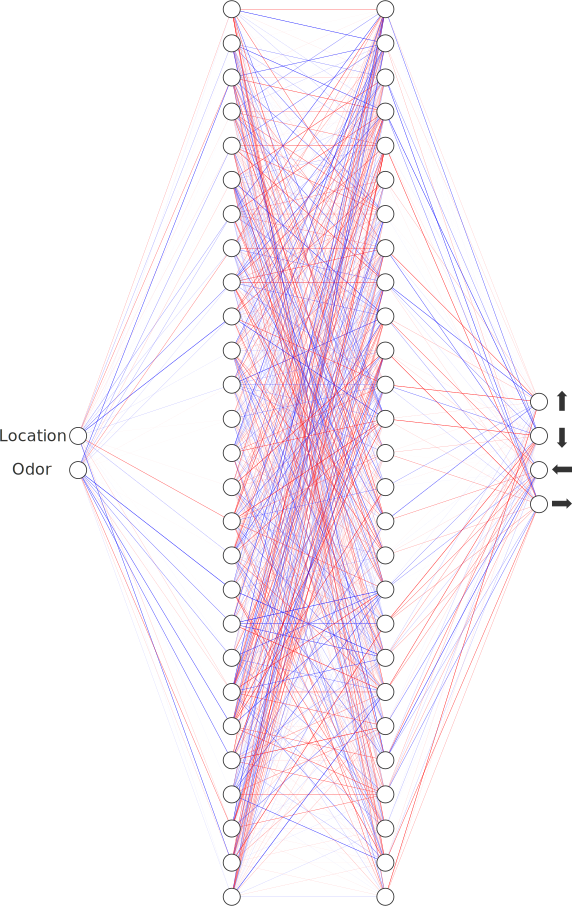
\includegraphics[height=6em]{./img/nn.svg.png}};
        \node [above=-0.2em of agent] {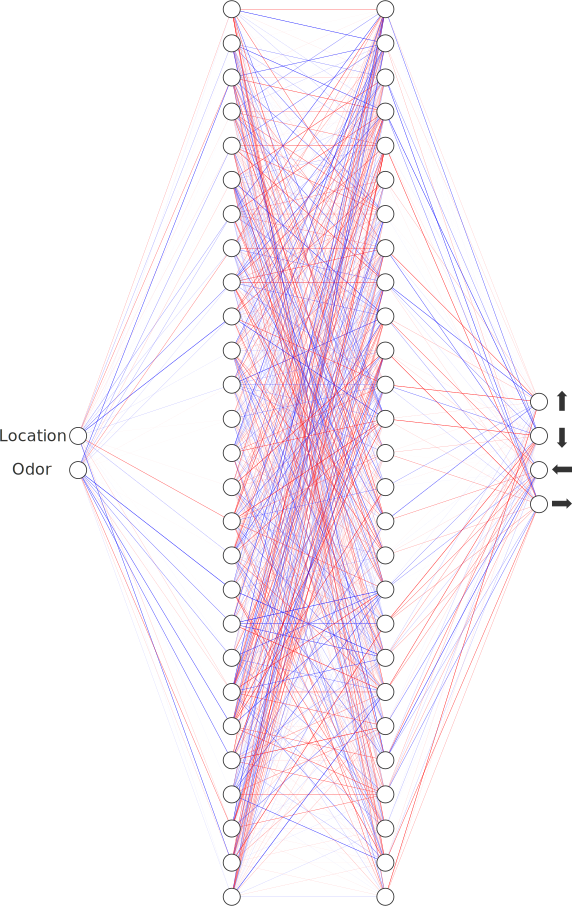
\includegraphics[height=8em]{./img/nn.svg.png}};
        \node[punkt,below=of center] (environment) {Environment \faIcon{globe}};
        \node[right=8em of center, align=center] (action) {Action\\$a_t$};
        \node[left=8em of center, align=center] (state_reward) {State, Reward\\$s_t$, $r_t$};
        \node [below=-0.2em of environment] {\includegraphics[height=8em]{./img/RL_env-allo-model.drawio.png}};

        \path[pil]
        (state_reward.east) edge [->, bend left=45] node {} (agent.west)
        (environment.west) edge [- , bend left=45] node {} (state_reward.east)
        (action.west) edge [->, bend left=45] node {} (environment.east)
        (agent.east) edge [-, bend left=45] node {} (action.west);
    \end{tikzpicture}
\end{adjustbox}
\end{frame}

\begin{frame}[label={sec:org8f938e3}]{What types of representations are in use to solve the odor-place association task ?}
\begin{columns}
\begin{column}[t]{0.5\columnwidth}
\begin{center}
Experiment
\end{center}
\begin{center}
\includegraphics[height=0.25\textheight]{img/place-cells-grid-cells.jpg.png}
\end{center}
\(\to\) Look for candidate patterns in the data: place cells, grid cells,\dots{}?
\end{column}
\begin{column}[t]{0.5\columnwidth}
\begin{center}
Simulation
\end{center}
\begin{center}
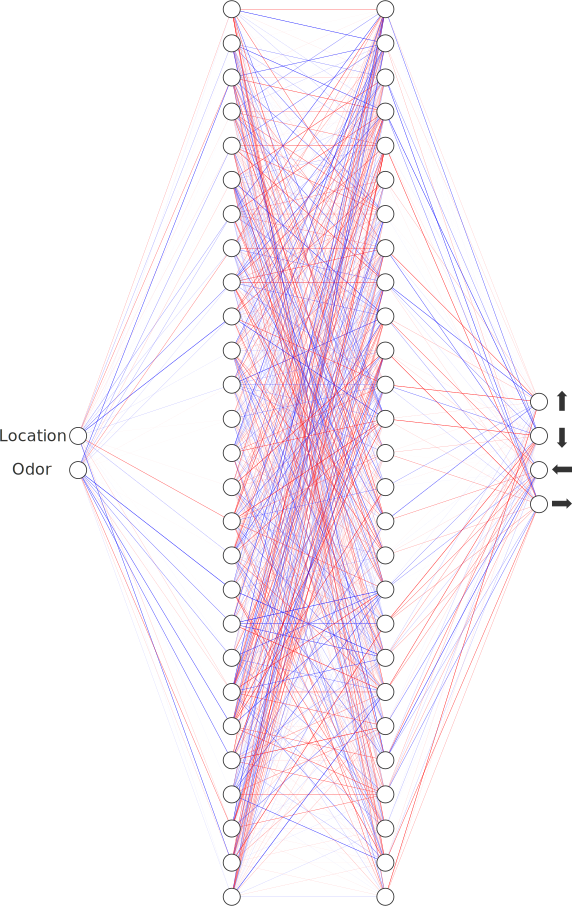
\includegraphics[height=0.25\textheight]{img/nn.svg.png}
\end{center}
\(\to\) Compare the data with the representations learned from scratch by the neural network

% \begin{textblock}{5}(-8.5,0.5)
% \begin{minipage}[t]{3em}
% \center
% \includegraphics[height=2em]{img/matt-nassar.jpg}\\
% \scriptsize
% Matt Nassar
% \end{minipage}
% \begin{minipage}[t]{3em}
% \center
% \includegraphics[height=2em]{img/niloufar-razmi.jpeg}\\
% \scriptsize
% Niloufar Razmi
% \end{minipage}
% \end{textblock}
\end{column}
\end{columns}
\end{frame}

\begin{frame}[<+->][label={sec:orgb96c776}]{Summary}
\begin{itemize}
\item We record in the LEC which encodes spatial \& olfactory information
\item Reinforcement Learning can be a useful tool to model behavior involving rewards and learning
\item The joint representation is needed to solve an odor-place location task
\end{itemize}
\end{frame}
\section*{Acknowledgments}
\label{sec:org016210d}
{%
\setbeamertemplate{background canvas}{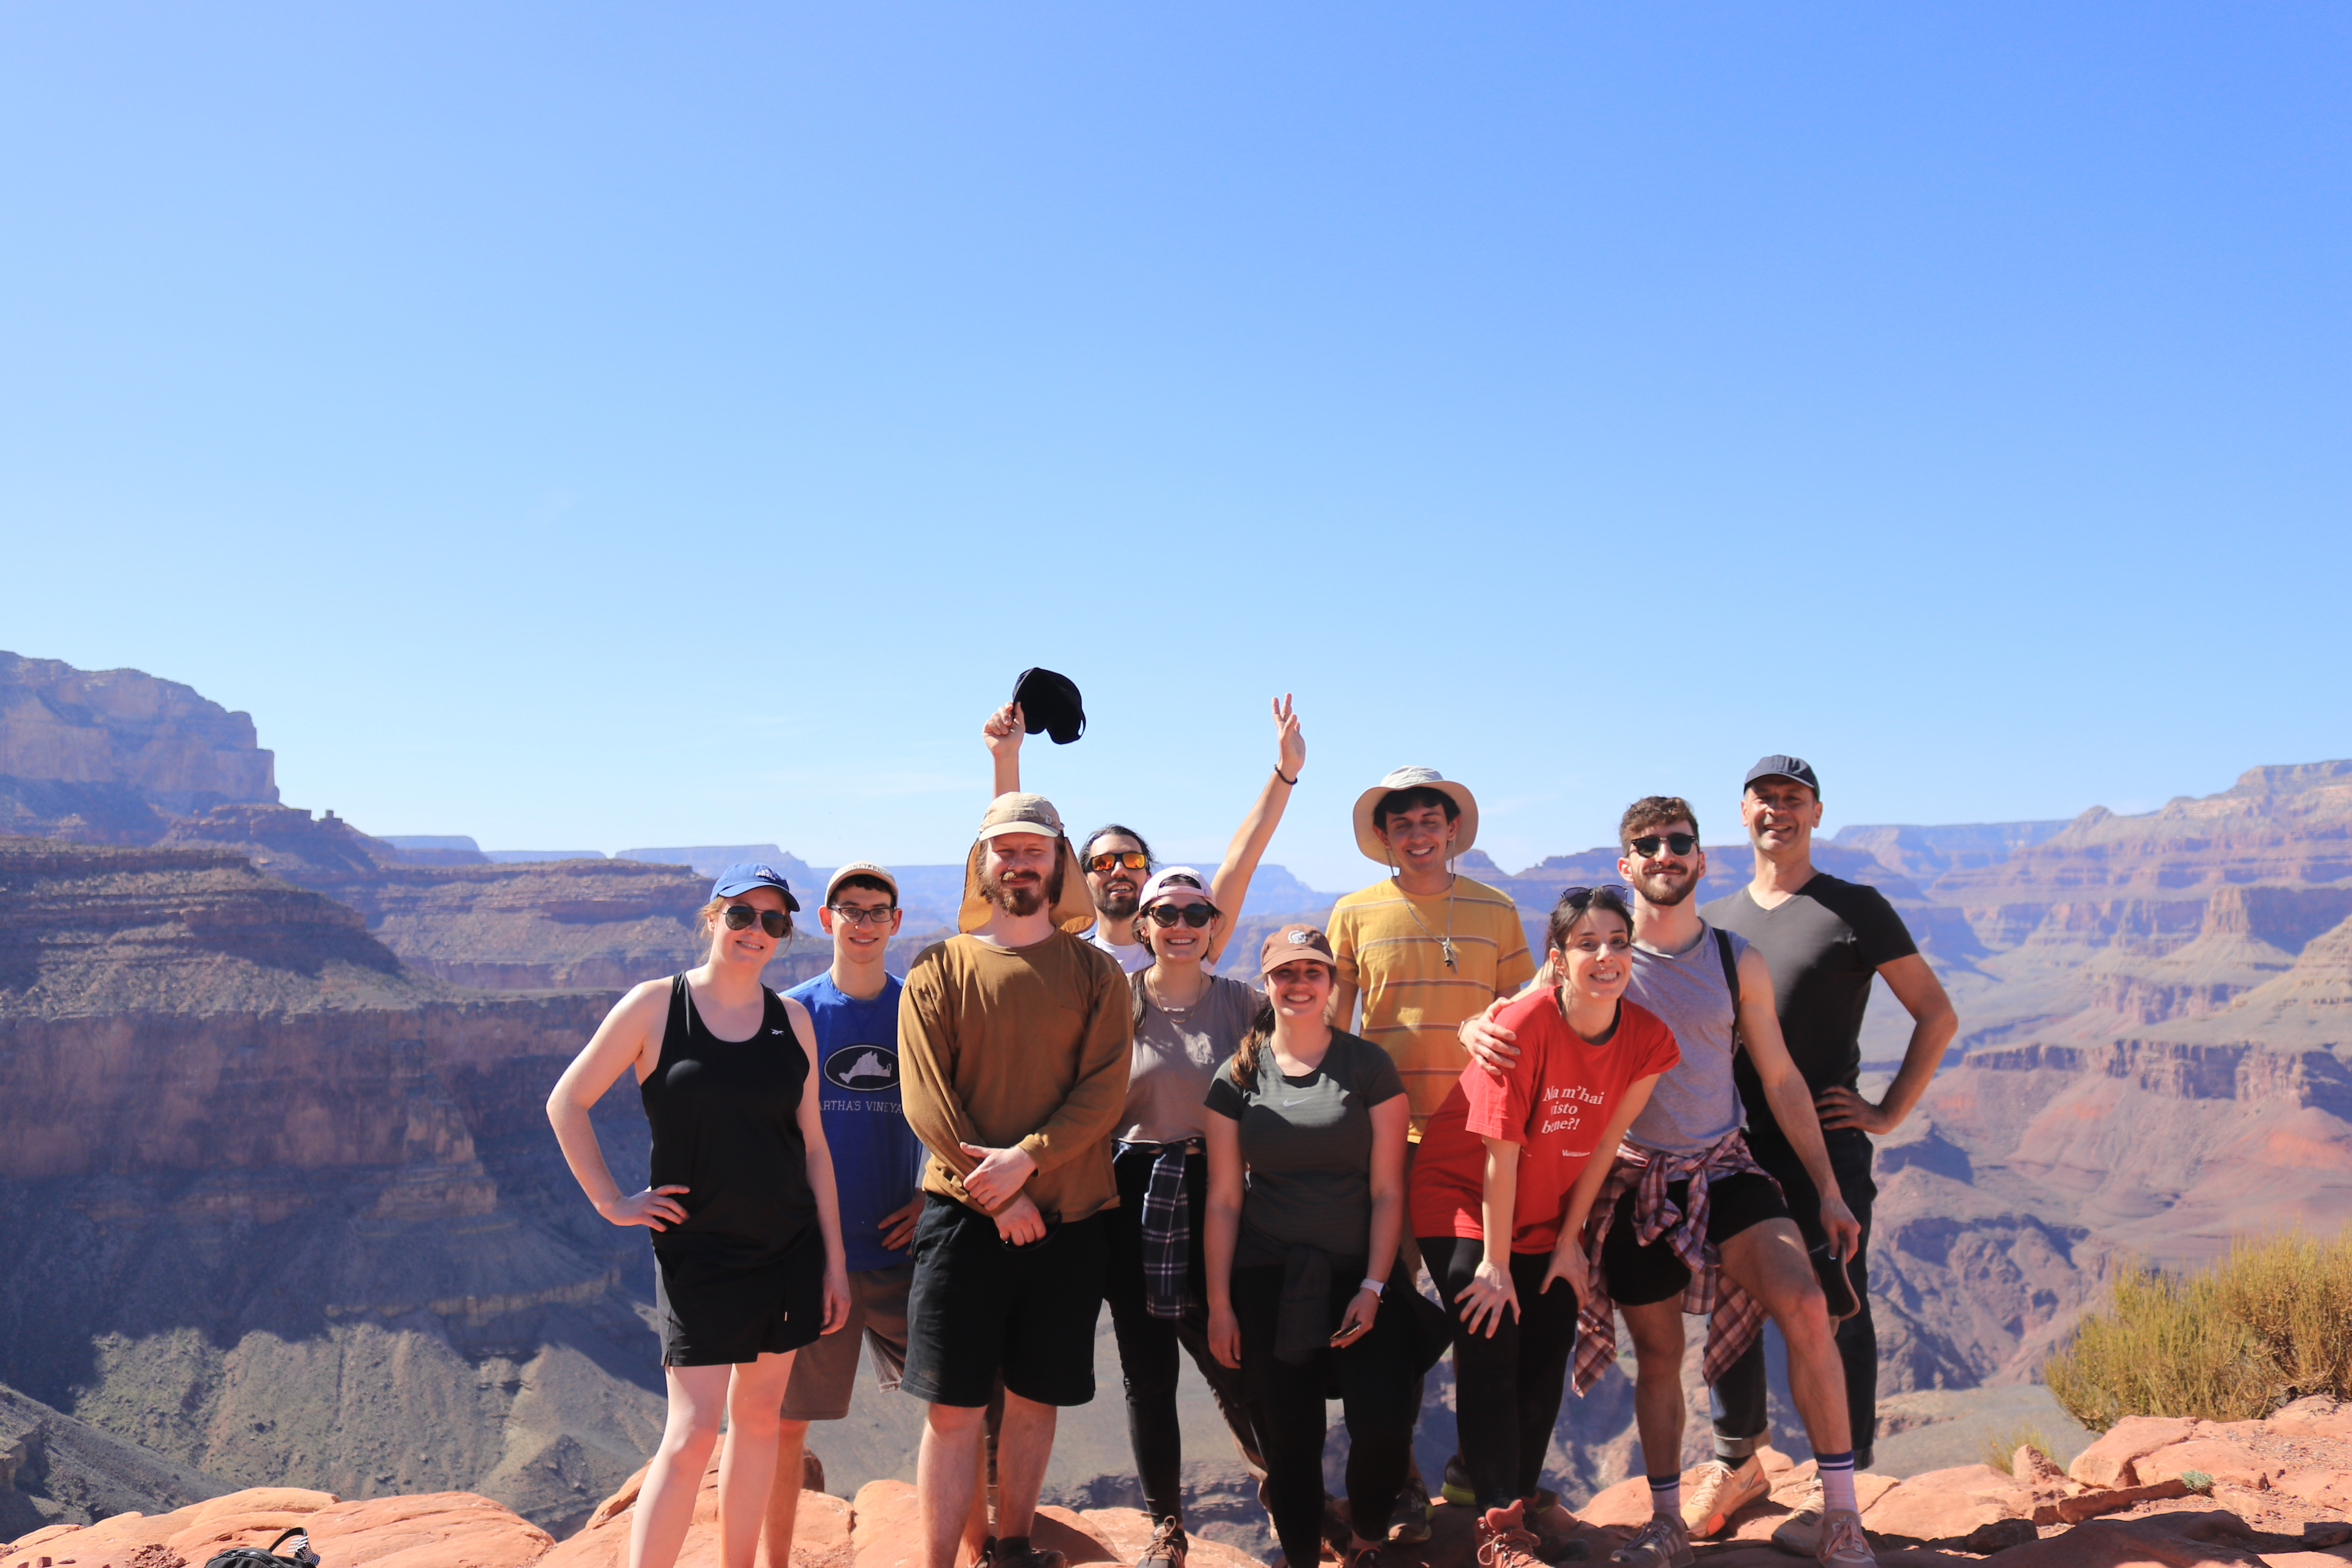
\includegraphics[height=\paperheight]{img/grand-canyon.JPG}}
\begin{frame}[fragile,t, plain]{Acknowledgments}
    \vspace{1em}
    \begin{columns}[T]
        \begin{column}{0.5\textwidth}
            \begin{itemize}
                \small
                \item Fleischmann lab
                \begin{itemize}
                    \tiny
                    \item Alexander Fleischmann
                    \item Keeley Baker
                    \item Olivia Mckissick
                    \item Tuan Pham
                    \item Simon Daste
                    \item Max Seppo
                    %\item \colorbox{white}{\transparent{0.2}Sara Zeppilli}
                    \item Sara Zeppilli
                    \item Nell Klimpert
                    \item Erin Meyers
                    \item Eseosa Uwaifo
                    \item Camille Donoho
                    \item Timothy Pyon
                \end{itemize}
            \end{itemize}
            \vspace{5em}
            \includegraphics[height=1.5cm]{img/qr-code.png}\\
            %\colorbox{white}{\footnotesize\transparent{0.5}https://reduced.to/tn9x6}
        \end{column}

        \begin{column}{0.5\textwidth}
            \begin{itemize}
                \small
                \item Collaborations
                \begin{itemize}
                    \tiny
                    \item Matt Nassar
                    \item Jason Ritt
                    \item Niloufar Razmi
                \end{itemize}
            \end{itemize}
        \end{column}
    \end{columns}
\end{frame}
}
\end{document}
